\chapter{Images}
\label{images}

% \begin{figure}
%     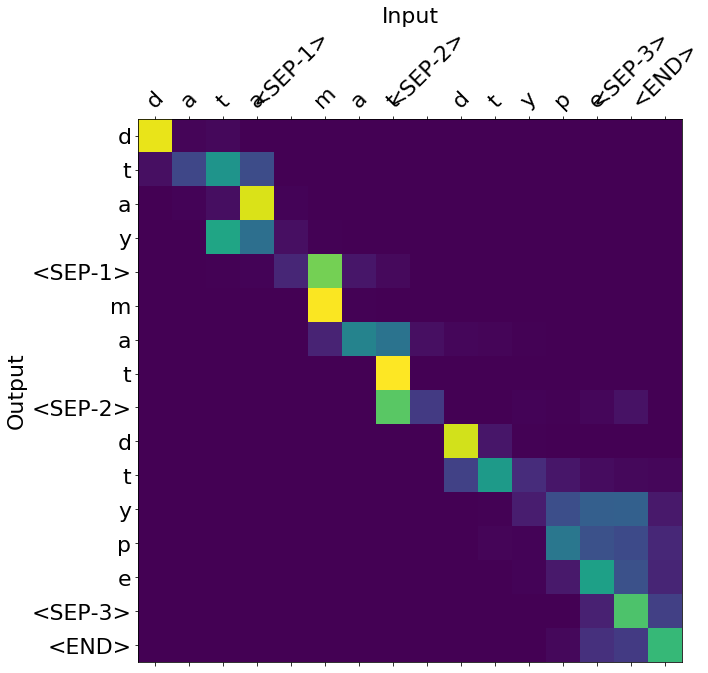
\includegraphics[width=0.8\linewidth]{images/typical_attention.png}
% \end{figure}

% \begin{table}
% \begin{center}
% \begin{tabular}{ | c || c |}
%     \hline
%     \hline
%     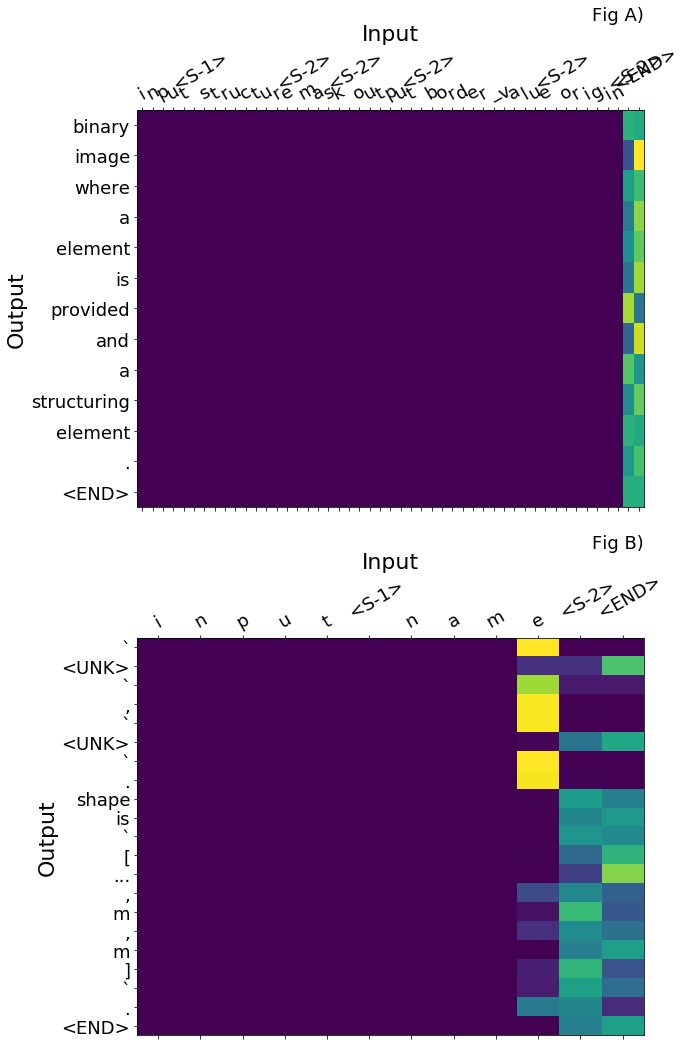
\includegraphics[width=0.5\linewidth]{images/otherargs_example.png}
%     &
%     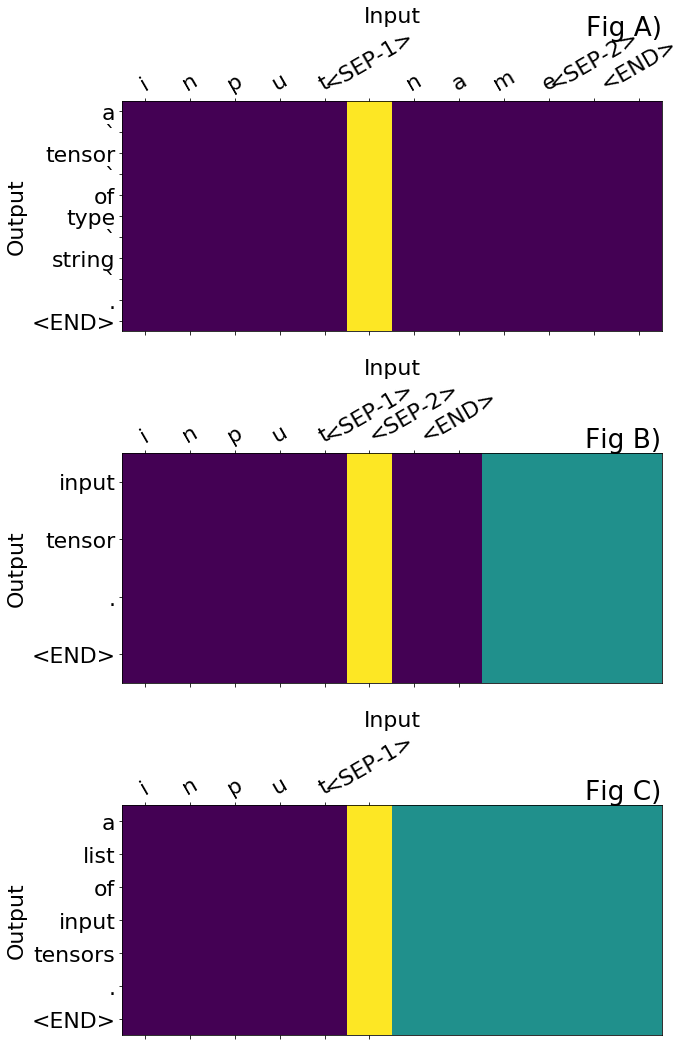
\includegraphics[width=0.5\linewidth]{images/different_translations_dupsXotherargs_3230minib.png} \\


%     \hline

%     \hline
% \end{tabular}
% \end{center}
% \end{table}



% \begin{table}
% \begin{center}
% \begin{tabular}{ l  }

% \textbf{Nonsense}\\

% \textbf{I}: \mintinline[]{python}{i n p u t <SEP-1> s t r u c t u r e <SEP-2> m a s k <SEP-2> o u t p}...\\
% ...\mintinline[]{python}{u t <SEP-2> b o r d e r _ v a l u e <SEP-2> o r i g i n <SEP-2> <END>}\\
% \textbf{D}: binary image to be propagated inside ` mask ` .\\
% \textbf{P}: binary image where a element is provided and a structuring element . $<$END$>$\\
% \\\hline\\


% \textbf{Overfitting}\\

% \textbf{I}: \mintinline[]{python}{e n c o d i n g _ t y p e <SEP-1> s e l f <SEP-2> d o c u m e}...\\
% ...\mintinline[]{python}{n t <SEP-2> r e t r y <SEP-2> t i m e o u t <SEP-2> <END>}\\
% \textbf{D}: the encoding type used by the api to calculate offsets .\\
% \textbf{P}: the encoding type used by the api to calculate sentence offsets . \\
% \\\hline\\




% \textbf{Underdetermination}\\

% \textbf{I}: \mintinline[]{python}{i n p u t <SEP-1> n a m e <SEP-2> <END>}\\
% \textbf{D}: a ` tensor ` of type ` complex64 ` . a complex64 tensor .\\
% \textbf{P}: ` $<$UNK$>$ ` , ` $<$UNK$>$ ` . shape is ` [ ... , m , m ] ` . \\
% \\\hline\\

% \\

% \end{tabular}

% \caption{Three examples of typical errors in the character Seq-to-Seq model.  In this case, the first example shows good use of data in the sequence but is nonsensical. The second is an example of overfitting where the predicted sentence is found in the dataset. The final case, multiple sequences such as these are found in the dataset, each with a different discription. Without looking at code, or function name (in this case) it is impossible to disambiguate and the model fails to make sense }
% \end{center}
% \end{table}

% \begin{table}
% \begin{center}
% \begin{tabular}{l}

% \hline
% \textbf{Validation Example}\\

% \textbf{I}: \mintinline[]{python}{i n p u t <SEP-1> s t r u c t u r e <SEP-2> m a s k <SEP-2> o u t p}...\\
% ...\mintinline[]{python}{u t <SEP-2> b o r d e r _ v a l u e <SEP-2> o r i g i n <SEP-2> <END>}\\
% \textbf{D}: binary image to be propagated inside ` mask ` .\\
% \textbf{P}: binary image where a element is provided and a structuring element . $<$END$>$\\
% \\\hline\\

% \textbf{Training Examples} starting \mintinline[]{yaml}{i n p u t <SEP-1> s t r u c t u r e}\\
% \textbf{I}: \mintinline[]{yaml}{i n p u t <SEP-1> s t r u c t u r e 1 <SEP-2> s t r u c t u r}...\\
% ...\mintinline[]{yaml}{e 2 <SEP-2> o u t p u t <SEP-2> o r i g i n 1 <SEP-2> o r i g i n 2 <SEP-2> <END>}\\
% \textbf{D}: binary image where a pattern is to be detected .\\
% \\
% \textbf{I}: \mintinline[]{yaml}{i n p u t <SEP-1> s t r u c t u r e <SEP-2> i t e r a t i o n s <SEP-2> o u t }...\\
% ...\mintinline[]{yaml}{p u t <SEP-2> o r i g i n <SEP-2> m a s k <SEP-2> b o r d e r _ v a l u e }\\
% ...\mintinline[]{yaml}{<SEP-2> b r u t e _ f o r c e <SEP-2> <END>}\\
% \textbf{D}: binary array\_like to be closed . non-zero ( true ) elements form the subset to be closed .\\
% \\
% \textbf{I}: \mintinline[]{yaml}{i n p u t <SEP-1> s t r u c t u r e <SEP-2> o u t p u t <SEP-2> o r}...\\
% ...\mintinline[]{yaml}{i g i n <SEP-2> <END>}\\
% \textbf{D}: n-dimensional binary array with holes to be filled\\
% \\
% \textbf{I}: \mintinline[]{yaml}{i n p u t <SEP-1> s t r u c t u r e <SEP-2> o u t p u t <SEP-2> <END>}\\
% \textbf{D}: an array-like object to be labeled . any non-zero values in ` input ` are counted as features...\\
% ...and zero values are considered the background .\\
% \\
% \textbf{I}: \mintinline[]{yaml}{i n p u t <SEP-1> s t r u c t u r e <SEP-2> i t e r a t i o n s <SEP-2> m a s k }...\\
% ...\mintinline[]{yaml}{<SEP-2> o u t p u t <SEP-2> b o r d e r _ v a l u e <SEP-2> o r i g i n <SEP-2>}\\
% ...\mintinline[]{yaml}{b r u t e _ f o r c e <SEP-2> <END>}\\
% \textbf{D}: binary image to be eroded . non-zero ( true ) elements form the subset to be eroded .\\
% \\
% \textbf{I}: \mintinline[]{yaml}{i n p u t <SEP-1> s t r u c t u r e <SEP-2> i t e r a t i o n s <SEP-2> m a s k}...\\
% ...\mintinline[]{yaml}{<SEP-2> o u t p u t <SEP-2> b o r d e r _ v a l u e <SEP-2> o r i g i n <SEP-2>}\\
% ...\mintinline[]{yaml}{b r u t e _ f o r c e <SEP-2> <END>}\\
% \textbf{D}: binary array\_like to be dilated . non-zero ( true ) elements form the subset to be dilated .\\
% \\



% \end{tabular}

% \caption{A validation example and the a selection of training points. Despite being a long sequence, }
% \end{center}
% \end{table}



% \begingroup
% \begin{table}
% \begin{center}
% 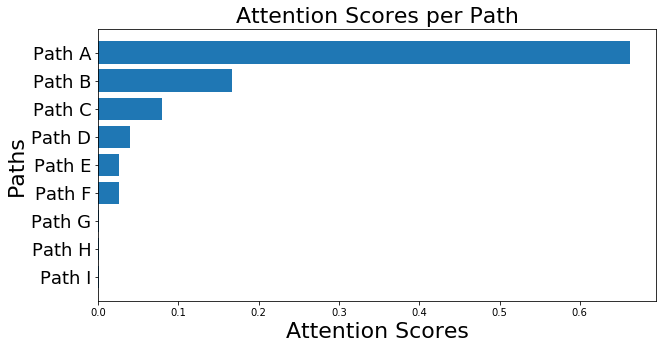
\includegraphics[width=0.8\linewidth]{ImagesCodeRelated/attention_xkcd.png}
%     \fontsize{10pt}{12pt}\selectfont
%         % how to set font size here to 10 px ?  
% \begin{tabular}{c l}
%     & \textbf{Paths} \\
%     \\
%     \textbf{Path A} & Name $\leftarrow$ comprehension $\leftarrow$ ListComp $\leftarrow$ Assign $\rightarrow$ Name : \mintinline[]{yaml}{palette} \\
%     \textbf{Path B} & Name $\leftarrow$ comprehension $\leftarrow$ ListComp $\leftarrow$ Assign $\leftarrow$ FunctionDef[...] \\
%         & [...]$\rightarrow$ Assign $\rightarrow$ ListComp $\rightarrow$ comprehension : \mintinline[]{yaml}{<UNK>} \\
%     \textbf{Path C} & $<$UNK$>$ : \mintinline[]{yaml}{color_palette} \\
%     \textbf{Path D} & Name $\leftarrow$ comprehension $\rightarrow$ Name : \mintinline[]{yaml}{name} \\
%     \textbf{Path E} & $<$UNK$>$ : \mintinline[]{yaml}{palette} \\
%     \textbf{Path F} & $<$UNK$>$ : \mintinline[]{yaml}{palette} \\
%     \textbf{Path G} & $<$UNK$>$ : \mintinline[]{yaml}{len} \\
%     \textbf{Path H} & $<$UNK$>$ : \mintinline[]{yaml}{name} \\
%     \textbf{Path I} & $<$UNK$>$ : \mintinline[]{yaml}{<UNK>} \\
% \end{tabular}
% \end{center}

% \caption{Example Attention Scores}
% \end{table}
% \endgroup

% \begin{listing}[h!] 
% 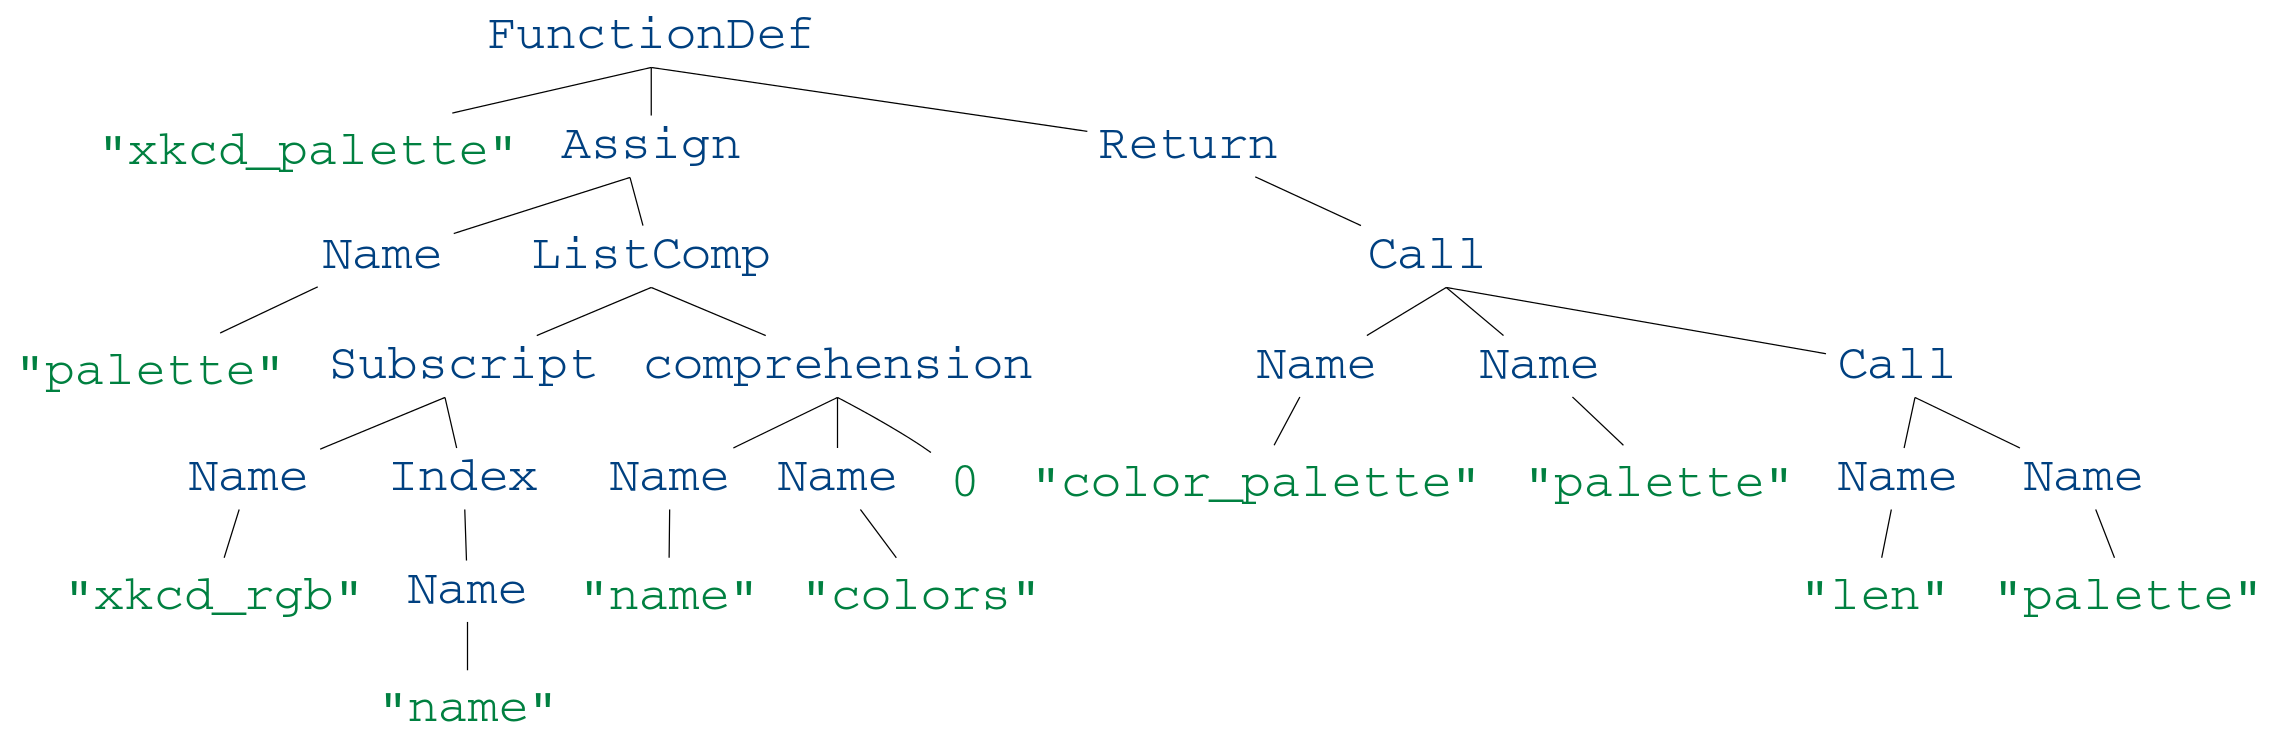
\includegraphics[width=0.8\linewidth]{ImagesCodeRelated/xkcd_palette_strip.png}
% \begin{minted}[]{python}
% def xkcd_palette(colors):
%     palette = [xkcd_rgb[name] for name in colors]
%     return color_palette(palette, len(palette))

% \end{minted}
% \begin{tabular}{l}
% \textbf{I}: \mintinline[]{python}{colors}\\
% \textbf{D}: list of keys in the `` seaborn.xkcd\_rgb `` dictionary .\\
% \textbf{P}: a list of data to read . if none , all other the first will be returned .\\
% \end{tabular}

% \caption{Code \& List}
% \end{listing}

% \begin{figure}
% \begin{center}
% 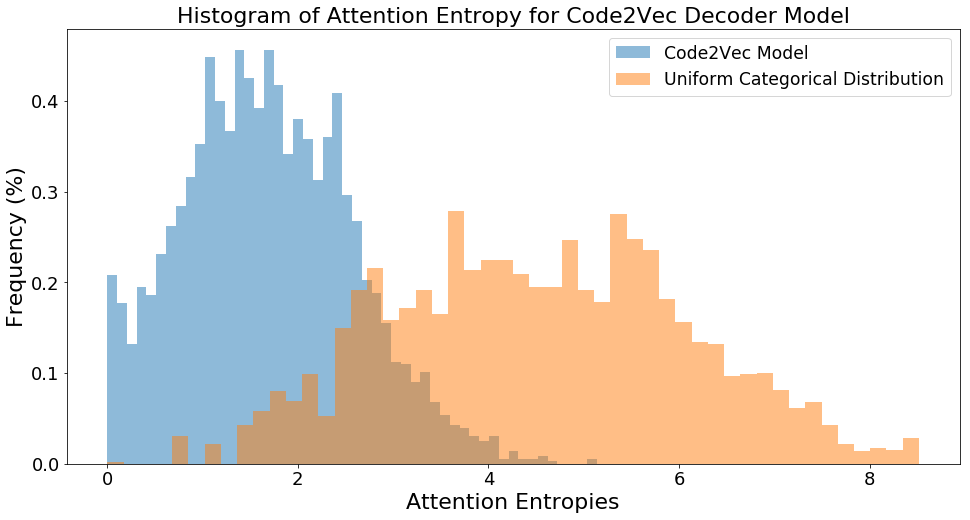
\includegraphics[width=.8\linewidth]{ImagesCodeRelated/code2vec_entropies.png}
% 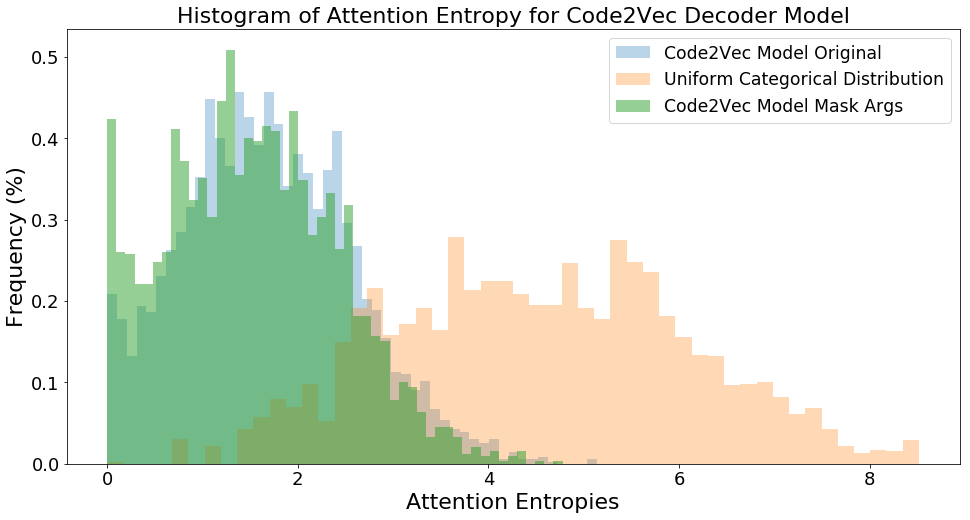
\includegraphics[width=0.8\linewidth]{ImagesCodeRelated/entropies_mask_args.png} 
% 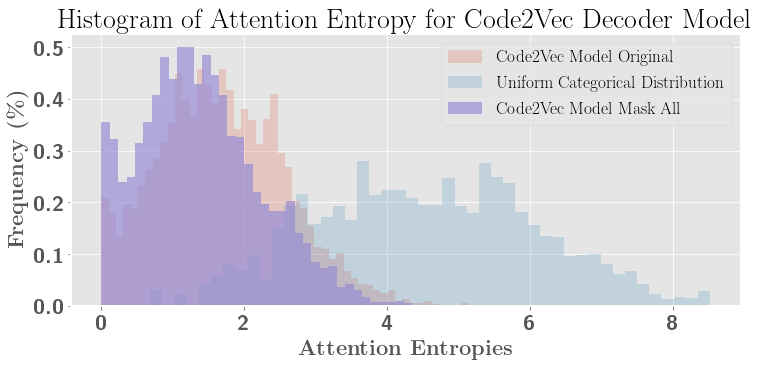
\includegraphics[width=0.8\linewidth]{ImagesCodeRelated/entropies_mask_all.png}
% 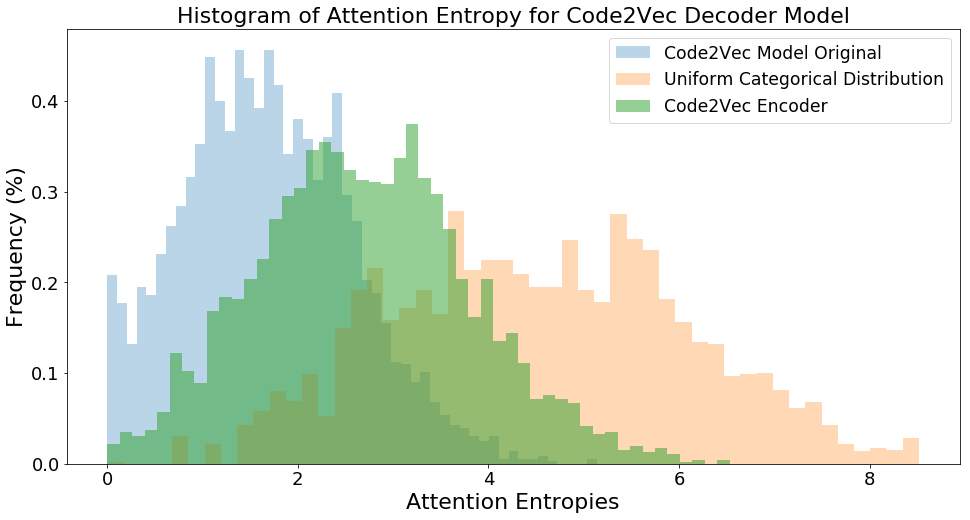
\includegraphics[width=.8\linewidth]{ImagesCodeRelated/save_c2e_encoder.png}
% \end{center}
% \end{figure}

\begin{table}
\begin{center}
\begin{tabular}{l}

\hline
\textbf{Rote Learner Hardest Code Only}\\
\\
\textbf{Random Sample of Bleu Scores} \\ 
\\
 
\textbf{BLEU4 (Sentence Level)}: 0.000
\textbf{Confidence}: 100.0\%  \\
\textbf{Argument}: \mintinline[]{python}{key_id}\\
\textbf{Description}: optional key id used to identify this private key . this can be useful to associate[...]\\
...the private key with its associated public key or certificate .\\
\textbf{Prediction}: string , uri for token endpoint . for convenience defaults to google 's endpoints but[...]\\
...any oauth 2.0 provider can be used . \\
\\
\textbf{B}: 0.000
\textbf{C}: 100.0\%  \\
\textbf{A}: \mintinline[]{python}{tensor_name_regex}\\
\textbf{D}: the regular-expression pattern of the name ( s ) of the x-tensor ( s ) to watch . x-tensor[...]\\
...refers to the tensors on the denominator of the differentiation .\\
\textbf{P}: a color string \\
\\
\textbf{B}: 0.000
\textbf{C}: 50.0\%  \\
\textbf{A}: \mintinline[]{python}{compile_ops}\\
\textbf{D}: whether to enable or disable compilation in the scope . either a python bool , or a callable[...]\\
 that accepts the parameter ` node\_def ` and returns a python bool .\\
\textbf{P}: ` str ` ( name ) , ` optimizer ` or ` function ` . optimizer to use . default : $<$UNK$>$ ' ( [...]\\
adaptive moment estimation ) . \\
\\
\hline\\
\textbf{A Random Sample of Bleu Scores $>0$ }\\\\ 


\textbf{B}: 0.047
\textbf{C}: 100.0\%  \\
\textbf{A}: \mintinline[]{python}{container}\\
\textbf{D}: ` bbox ` is positioned ; it defaults to the initial : class : ` bbox ` .\\
\textbf{P}: $<$UNK$>$ ' or $<$UNK$>$ ' . in $<$UNK$>$ ' mode , the channels dimension ( the depth ) is at[...]\\
 index 1 , in $<$UNK$>$ ' mode it is at index 3. it defaults to the ` $<$UNK$>$ ` value found in your keras[...]\\
  config file at ` $<$UNK$>$ ` . if you never set it , then it will be `` $<$UNK$>$ '' . \\
\\
\textbf{B}: 1.000
\textbf{C}: 100.0\%  \\
\textbf{A}: \mintinline[]{python}{weight}\\
\textbf{D}: if none , all edge weights are considered equal . otherwise holds the name of the edge[...]\\\
...attribute used as weight .\\
\textbf{P}: if none , all edge weights are considered equal . otherwise holds the name of the edge[...]\\\
...attribute used as weight . \\
\\
\textbf{B}: 0.344
\textbf{C}: 100.0\%  \\
\textbf{A}: \mintinline[]{python}{time}\\
\textbf{D}: either the name of the field corresponding to time in the data dataframe or x values[...]\\\
...for a plot when data is an array . if a series , the name will be used to label the x axis .\\
\textbf{P}: either the name of the field corresponding to the data values in the data $<$UNK$>$[...]\\\
...( i.e . the y coordinate ) or a string that forms the y axis label when data is an array . \\

\end{tabular}
\end{center}
\end{table}


\begin{enumerate}
    \item With the code lstm we see some of the behaviour we like, but also, only overfitting. There is no sequence so in some cases, a path or a single variable can be informative, but it performs well.
    \item See a single example and distribution of attention.
    \item CLearly there are a lot of spikes compared to uniform. More masking the more spiking, though this is partly due to best bleu. Compare at cross entropy time?
    \item Then look at, bleu per sentence, maybe av bleu per sentence per attn entropy.
    \item Big COMPARE vs ROTE LEARNER - can we conclude this is worth more researcg?
    \item Cna show how choices change w model for given example??

    \item C2VEnc: does combining add anythin? More capacity, check weights.
\end{enumerate}



% \begin{figure}
% \begin{center}
% 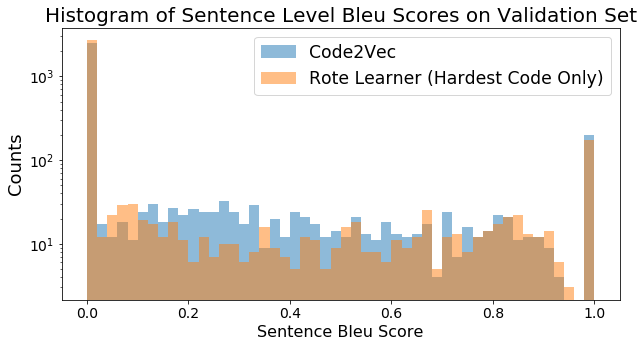
\includegraphics[width=0.8\linewidth]{ImagesCodeRelated/SentenceBleuCodeonly.png}
% 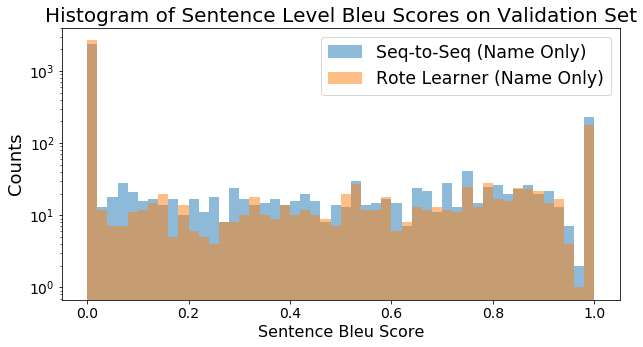
\includegraphics[width=.8\linewidth]{ImagesCodeRelated/SentenceBleuNameOnly.png}
% 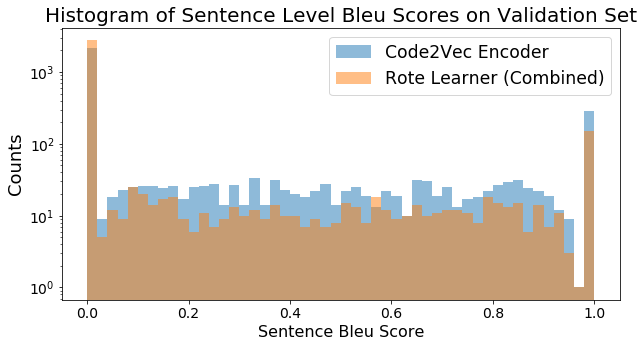
\includegraphics[width=.8\linewidth]{ImagesCodeRelated/SentBleuCombined.png}
% \end{center}
% \end{figure}



\begin{table}
\begin{center}
\begin{tabular}{l}


\hline
\textbf{Rote Learner Otherargs Only}\\
\\
\textbf{A Random Sample of Bleu Scores  } \\

 
\textbf{B}: 0.000
\textbf{C}: 100.0\%  \\
\textbf{Argument}: \mintinline[]{python}{k e y _ i d <SEP-1> p r i v a t e _ k e y <END>}\\
\textbf{D}: optional key id used to identify this private key . this can be useful to associate the private key with its associated public key or certificate .\\
\textbf{P}: string . password for $<$UNK$>$ \# 12 key . \\
\\
\textbf{B}: 0.581
\textbf{C}: 100.0\%  \\
\textbf{Argument}: \mintinline[]{python}{o u t <SEP-1> i m a g e <SEP-2> s e l e m <SEP-2> m a s k <SEP-2> s h i f}...\\
...\mintinline[]{python}{t _ x <SEP-2> s h i f t _ y <END>}\\
\textbf{D}: if none , a new array is allocated .\\
\textbf{P}: if none , a new array will be allocated . \\
\\
\textbf{B}: 0.000
\textbf{C}: 5.3\%  \\
\textbf{Argument}: \mintinline[]{python}{t e n s o r _ n a m e _ r e g e x <SEP-1> s e l f <SEP-2> g r a p h <END>}\\
\textbf{D}: the regular-expression pattern of the name ( s ) of the x-tensor ( s ) to watch . x-tensor refers to the tensors on the denominator of the differentiation .\\
\textbf{P}: an $<$UNK$>$ of $<$UNK$>$ . items can be an instance of $<$UNK$>$ , $<$UNK$>$ , or $<$UNK$>$ . \\
\\
\textbf{B}: 0.000
\textbf{C}: 25.0\%  \\
\textbf{Argument}: \mintinline[]{python}{c o m p i l e _ o p s <SEP-1> s e p a r a t e _ c o m p}...\\
...\mintinline[]{python}{i l e d _ g r a d i e n t s <END>}\\
\textbf{D}: whether to enable or disable compilation in the scope . either a python bool , or a callable that accepts the parameter ` node\_def ` and returns a python bool .\\
\textbf{P}: dictionary mapping variable names of the regular grammar to the $<$UNK$>$ that should be used for this part . ( this can call other $<$UNK$>$ recursively . ) if you wish a part of the grammar to just get one token , use a ` $<$UNK$>$ ` . \\
\\
\hline\\
\textbf{A Random Sample of Bleu Scores $>0$  }\\
\\

\textbf{B}: 0.581
\textbf{C}: 100.0\%  \\
\textbf{Argument}: \mintinline[]{python}{o u t <SEP-1> i m a g e <SEP-2> s e l e m <SEP-2> m a s k <SEP-2> s h i f}...\\
...\mintinline[]{python}{t _ x <SEP-2> s h i f t _ y <END>}\\
\textbf{D}: if none , a new array is allocated .\\
\textbf{P}: if none , a new array will be allocated . \\

\textbf{B}: 0.142
\textbf{C}: 100.0\%  \\
\textbf{Argument}: \mintinline[]{python}{x <SEP-1> y <SEP-2> i n i t _ m e a n <SEP-2> i n i t _ s t d d e v <END>}\\
\textbf{D}: tensor or placeholder for input features .\\
\textbf{P}: tensor or placeholder for labels ( $<$UNK$>$ ) , shape should be [ $<$UNK$>$ , $<$UNK$>$ ] . \\

\textbf{B}: 0.071
\textbf{C}: 25.0\%  \\
\textbf{Argument}: \mintinline[]{python}{o r i g i n <SEP-1> s e l f <SEP-2> X <SEP-2> c m a p <SEP-2> n o r m <SEP-2> a}...\\
...\mintinline[]{python}{s p e c t <SEP-2> i n t e r p o l a t i o n <SEP-2> a l p h a <SEP-2> v m i n <SEP-2> v m a x <SEP-2> e x t e n t <SEP-2> s h a p e <SEP-2> f i l t e r n o r m <SEP-2> f i l t e r r a d <SEP-2> i m l i m <SEP-2> r e s a m p l e <SEP-2> u r l <SEP-2> d a t a <SEP-2> k w a r g s <END>}\\
\textbf{D}: place the [ 0,0 ] index of the array in the upper left or lower left corner of the axes . if none , default to rc ` image.origin ` .\\
\textbf{P}: if $<$UNK$>$ ' , changes the image aspect ratio to match that of the axes . \\

\end{tabular}
\end{center}
\end{table}
